\chapter{Methodology}

\section{First-Principles Calcualtions}

In this disseration, the ground state energy structures, thermodynamic propertie and mechanical properties are calcualted using first-principles based on Density Functional Theory. The first-priniciples refers to the calculations orginating from first-principles, meaning that the inputs are the atomic coordinates and atomic numbers. This method computes the interactions between atoms in a periodic supercell. This is determined using quantum mechanical electronic theroy that is based on the electronic charge density. do not rely on any emprical data. This section provides a description of the DFT methodology.

Schr$\ddot{o}$dinger's time-independent non-relativisitc equation is a solution to the many-body problem of calculating the interactions of postiviely charged nuclei and negatively charged electrons. The Schr$\ddot{o}$dinger equation:

%%
\begin{equation}
\label{eq: schrodinger}
\left[ \sum_{i=1}^{N} \left( - \frac{\hbar^2}{2m} \nabla_{i}^2 + V_{ext} (r_{i}) \right) + \sum_{i<j} U (r_{i}, r_{j}) \right] \Psi = E \Psi
\end{equation}
%%

\noindent where $\Psi$ describing the wave function of electrons, $E$ describes the systems energy and the first part representing the Hamiltonian ($\hat{H}$). The $\hat{H}$ of the system is described by three parts, the first part representing the kinetic energy with $N$ being the total number of electons in the system, $\hbar$ being Planck's constant and $m$ the mass of a electron. The second term $V_{ext}$ gives the external potential and $U$ is the potential of the electron-electron repulsion. 

Eq. \ref{eq: schrodinger} can be solved for $\Psi$ with the lowest energy $E_0$ being the ground state energy. Assuming the nuclei-nuclei interactions are neglected due to the Born-Oppenheimer approximation which allows us to assume the nuclei are stationary and ignore the motion of nuclei on the electronic timescale. This assumption is due to the mass difference, with nuceli being \~ 10$^3$ to 10$^5$ larger than electrons. However, even with approximations solving Eq. \ref{eq: schrodinger} difficult to deal with due to the electron-electron Columb interactions making the electronic motion correlated and the fact that the many-body problem results in too many variables because of the 3N degrees of freedom. 

Hohenberg-Kohn formulated two thereoms to simplify this problem \cite{Hohenberg1964}. The first theorem is that the external potential as a unique functional of the electron density. The second thereom states that the density that minimizes the total energy is the exact ground state density and thus the ground state is obtained variationaly. With these thereoms, Kohn-Sham proved that the problem can be solved as if the electrons are not interacting and still obtain the density as if they were with their equation \cite{Kohn1965}:
 
  \begin{equation}
 \label{eq: kohnsham}
\left[ -\frac{\hbar^2}{2m} \nabla^{2} + V_{ext} (r) + V_{Hartree}(r) + V_{XC} (r) \right] \phi_{1}(r) = \epsilon_{i} \psi_{i}(r)
 \end{equation}
 %%
 
 \noindent where $V_{ext}(r)$ is described the electron-nuclei interaction similar as in Eq. \ref{eq: schrodinger}:

\begin{equation}
\label{eq: vext}
V_{ext} = - e^2 \sum_{a} \frac {Z_{a}}{|r_i - R_a|}
\end{equation}

\noindent where $r_i$ represents the position of electron i and $R_a$ represents the position of nucleus $a$ with a charge valance of $Z_a$. The electron-electron interactions are represented by $V_{Hartree}$:

\begin{equation}
\label{eq: vhartree}
V_{Hartree} (r) = e^{2} \int \frac {\rho(r)}{|r - r_{j}|} d^3r
\end{equation}
%%

\noindent where $r$ and $r_j$ represent the electrons and $\rho (r)$ is described by :

\begin{equation}
\label{eq: rhop}
\rho (r) = \sum_{i}^N | \psi_{i} (r) |^2
\end{equation}
%%

\noindent The final term of $V_{xc}$ is the exchange correlation potential that is described in terms of an exchange-correlation energy. By implementing th thereoms and the Kohn-Sham equation, the energy of the system can be calculated. 

While there is no exact solution to the exchange-correlation (X-C) energy avaliable, there are multiple different appoximations. Each approximation is done to account for different things. In the present work, the generalized gradient approximation by Perdew and Wang (PW91) \cite{Perdew1992} and the generalized gradient approximation by Perdew, Burke and Ernzerhoff (PBE) \cite{Perdew1996a} where used. The generalized gradient approach impoves the total energies, atomization ernegies as opposed to other methods such as the local density approximation \cite{Ceperley1980} but can over-correct for the expansion and softening of bonds. The generalized gradient approximation (GGA) is favored for densities that are inhomogenous. Based on previous research done by Perdew et al. \cite{Perdew1996a}, GGA's are considered to be adequate approximations for calculating metals. The use of PW91 vs PBE was compared when looking at the elastic properties of the Ti-Ta system. The results showed little difference in calcluated elastic properites. The PW91 X-C functional was designed to satisfy as many exact conditions as possible and thus has some issues. Perdew introduced the PBE X-C functional as an improvement to PW91 which satisfied less exact conditions and only looked at the ones that were energtically significant for metals. Due to this and the fact the results vary so little, the PBE X-C functional was chosen to be used for the present thesis work.  



\subsection{Density Functional Theory at 0 $^\circ$K}

 The ground state energy at 0 $^\circ$K with the contribution of zero-point vibrational energy can be calcaulted by using the equation of states fitting for the relationship between the energy and volume of the structure. The EOS fitting is achieved through an energy-volume ($E_{0}-V$) curve of 5 or more relaxed volumes and using the four-parameter Birch-Murnaghan (BM4) EOS \cite{Shang2010}:

%%
\begin{equation}
\label{eq: zeroenergy}
E_{0}(V) = a + bV^{\frac{-2}{3}} + cV^{{-4}{3}} + dV^{-2}
\end{equation}
%%

\noindent where $a$, $b$, $c$ and $d$ are fitting parameters. From this, the volume $V_0$, ground state energy $E_{0}$, bulk modulus $B_{EOS}$, and first derviative with respect to pressure $B'$ can be calculated. 

From the ground state energies, the energy of formation and enthalpy of formation at 0 $^\circ$K can be calculated by finding the differenc between the structures energy and a reference state, normally the standard element reference state at standard pressure and temperature. The valance configuration for each element was selected based on the VASP recommendations. The p electrons were treated as valance for the Mo and Ta, the d electrons were treated as valance for Sn and the s electrons were treated as valance for Ti, Nb, and Zr \cite{Kresse1996,Kresse1999}. 

\subsection{Finite-temperature thermodynamics}

The Helmholtz energy, F (V,T) can be calulated, with DFT, as a function of temperature $T$ and volume $V$:
 %%
 \begin{equation}
 \label{eq: helmholtz}
 F(V,T) = E_{0}(V) + F_{vib}(V,T) + F_{T-el}(V,T)
 \end{equation}
 %%
 
 \noindent where $E_0$ is the static contribution at 0 $^\circ$K without the contribution of zero-point vibrational energy, $F_{vib}$ is the temperature-dependent vibrational contribution, and $F_{T-el}$ is the thermal electronic contribution. At ambient pressure, the Helmholtz energy of the system is equal to the Gibbs energy, which is used in the CALPHAD modeling. The vibrational contribution is obtained through the phonon quasiharmonic supercell (phonon approach) or the Debye-Grüneisen method (Debye). The phonon approach is a more accurate approach compared to the Debye model but it is also more computationally expensive. In the present work both the phonon and Debye models are used in different sections. The vibrational contribution is obtained through phonon calculations of at least five different volumes \cite{Wang2012}: 

%%
\begin{equation}
\label{eq: phonon}
F_{vib}(V,T) = k_{b}T \int_{0}^{infty} ln[2sinh\frac{\hbar \omega}{2k_BT}] g(\omega) d\omega
\end{equation}
%%

\noindent where $g(\omega)$ is the phonon density of states as a function of phonon frequency $\omega$ at volume $V$.  In addition, the Debye model is used to estimate the vibrational contribution \cite{Shang2010}: 

%%
\begin{equation}
\label{eq: debye}
F_{vib}(V,T) = \frac{9}{8} k_{b} \theta_{D}(V) - k_{B}T[D (\frac{\theta_D(V){T}}) + 3ln(1-e^{\frac{-\theta_{D}(V)}{T}})] 
\end{equation}
%%

\noindent where $\theta_{D}$ is the Debye temperature, $T$ is the temperature, and $D[\frac{\theta{D}(V)}{T}]$ is the Debye function. The Debye temperature is calculated through: 

%%
\begin{equation}
\label{eq: debyetemp}
\theta_{D} = s \frac{(6\pi^2)^{\frac{1}{3}}\hbar}{k_B} V_{0}^{\frac{1}{6}} (\frac{B}{M})^{\frac{1}{2}} (\frac{V_0}{V})^{\gamma} 
\end{equation}
%%

\noindent where $s$ is the Debye temperature scaling factor, $\gamma$ is the Grüneisen parameter determined by the pressure derivative of bulk modulus ($B'$), $B$ is the bulk modulus, $M$ is the atomic mass, and $V_0$ is the equilibrium volume. Here the equilibrium properties $V_0$, $B$, and $B'$ are estimated from the EOS of Eq. Y. The Debye temperature scaling factor was determined by Moruzzi et al. \cite{Moruzzi1988} to be 0.617 for nonmagnetic metals. However, this value has been shown to be less accurate for other materials. Liu et al. extensively looked at the Debye scaling factor and how to calculate the scaling factor based on a the Poisson’s ratio of a material \cite{Liu2015}. The methodology by Liu et al. \cite{Liu2015} was used for the present work to calculate the scaling factor: 

%%
\begin{equation}
\label{eq: debyescaling}
s(\nu) = 3^{\frac{5}{6}} [4\sqrt{2} (\frac{1 + \nu}{1 - \nu})^{\frac{3}{2}} + (\frac{1 + \nu}{1 - \nu})^{\frac{-1}{3}}]
\end{equation}
%%

\noindent where $\nu$ is the Poisson’s ratio, which can be calculated from the elastic stiffness constants.

The thermal electronic contribution is based on the electronic density of states and calculated with the Fermi-Dirac statistics \cite{Shang2010,Wang2004}:

%%
\begin{equation}
\label{eq:thermalelectronic}
F_{T-el} = E_{T-el} - T S_{T-el}
\end{equation}
%%

The $E_{ele}$ and $S_{ele}$ represent the energy and entropy of the thermal electron excitations, respectively. The $E_{T-el}$ is expressed by:

%%
\begin{equation}
\label{eq:etel}
E_{T-el} (V,T) = \int n\left(\epsilon, V\right) f \left(\epsilon, T\right) \epsilon d \epsilon - \int^{\epsilon_{f}} n (\epsilon) \epsilon d \epsilon
\end{equation}
%%

\noindent and the entropy $S_{T-el}$ is expressed by:

%%
\begin{equation}
\label{eq:sel}
S_{T-el} (V,T) = -k_{B} \int n(\epsilon, V) \left[ ln f \left(\epsilon,T\right) + \left( 1 - f(\epsilon, T) \right) ln \left( 1 - f \left(\epsilon, T \right) \right) \right] d\epsilon 
\end{equation}
%%

\noindent where $n(\epsilon, V)$ is the electronic density of states (DOS) at energy $\epsilon$,  $f (\epsilon,T)$ is the Fermi-Dirac distribution, $\epsilon_{f}$ is the Fermi energy level and $k_{B}$ is Boltzmann's constant. The Fermi-Dirac distribution $f (\epsilon, T)$ is expressed by:

%%
\begin{equation}
\label{eq:fermidirac}
f (\epsilon,T) = \left[ exp \left( \frac{\epsilon - \mu}{k_{B} T} \right) + 1 \right]^{-1}
\end{equation}
%%

and $\mu$ is the chemical potential of the electrons. The $S_{T-el}$ entropy term is expressed by:



\subsection{Elastic stiffness calculations}

The single crystal elastic stiffness constants $c_{ij}'s$ were calculated from the ground state energy structure using a stress-strain method developed by Shang et al. \cite{Shang2007c}. With this method, a set of independent strains $\varepsilon = (\varepsilon_{1}, \varepsilon_{2}, \varepsilon_{3}, \varepsilon_{4}, \varepsilon_{5}, \varepsilon_{6})$  were imposed on the crystal lattice, where $\epsilon_{1}$, $\epsilon_{2}$, and $\varepsilon_{3}$ are the normal strains, $\varepsilon_{4}$, $\varepsilon_{5}$, and $\varepsilon_{6}$ the shear strains, and a set of stresses $\sigma = (\sigma_{1}, \sigma_{2}, \sigma_{3}, \sigma_{4}, \sigma_{5},\sigma_{6})$ are generated. Hooke's law was used to calculate the elastic stiffness constants: 

%%
\begin{equation}
\label{eq: hookes}
\begin{pmatrix}
	c_{11} & c_{12} & c_{13} & 0 & 0 & 0\\
	c_{12} & c_{22} & c_{23} & 0 & 0 & 0\\
	c_{13} & c_{23} & c_{33} & 0 & 0 & 0\\
	0 & 0 & 0 & c_{44} & 0 & 0\\
	0 & 0 & 0 & 0 &  c_{55} & 0\\
	0 & 0 & 0 & 0 & 0 & c_{66} \\    		
\end{pmatrix} =
\begin{pmatrix}
	\varepsilon_{1,1} & & \varepsilon_{1,n}\\
	\varepsilon_{2,1} & & \varepsilon_{2,n}\\
	\varepsilon_{3,1} & ... & \varepsilon_{3,n}\\
	\varepsilon_{4,1} & & \varepsilon_{4,n}\\
	\varepsilon_{5,1} & & \varepsilon_{5,n}\\
	\varepsilon_{6,1} & & \varepsilon_{6,n}\\					
\end{pmatrix}^{-1}
\begin{pmatrix}
	\sigma_{1,1} & & \sigma_{1,n}\\
	\sigma_{2,1} & & \sigma_{2,n}\\
	\sigma_{3,1} & ... & \sigma_{3,n}\\
	\sigma_{4,1} & & \sigma_{4,n}\\
	\sigma_{5,1} & & \sigma_{5,n}\\
	\sigma_{6,1} & & \sigma_{6,n}\\					
\end{pmatrix}
\end{equation}
%%

where “-1” represents the pseudo-inverse. Due to symmetry, the bcc structure only has three independent elastic stiffness constants. However, with a lack of bcc stability for some of the calculations, all of the elastic stiffness constants are calculated and the average $\overline{C}_{11}$, $\overline{C}_{12}$ and $\overline{C}_{44}$ values are calculated:

%%
\begin{equation}
\label{eq: averagec11}
\overline{C}_{11} = \frac{(c_{11} + c_{12} + c_{44})}{3}
\end{equation}
%%

%%
\begin{equation}
\label{eq: averagec12}
\overline{C}_{12} = \frac{(c_{12} + c_{13} + c_{23})}{3}
\end{equation}
%%

%%
\begin{equation}
\label{eq: averagec44}
\overline{C}_{44} = \frac{(c_{44} + c_{55} + c_{66})}{3}
\end{equation}
%%

This case is for the unstable bcc elastic calculations to mimic the behavior of a cubic structure. The largest variance between the similar elastic stiffness constants, when calculating the average, is used to show the deviation from the bcc symmetry in the calculations shown as error bars. The stable bcc structures shows no variance and thus no error bars. To examine the effects of different strain on the elastic properties, three groups of non-zero strain magnitudes of $\pm$0.01, $\pm$0.03, and $\pm$0.07 are tested in chapter 5 and it can be noted that the results have negligible changes with respect to the three groups of strains tested herein. Therefore, $\pm$0.01 are used for all the calculations. The calculated elastic stiffness constants are used to calculate the polycrystalline elastic properties including bulk (B), shear (G), and Young’s (E) modulus using the Voigt-Reuss-Hill (VRH) approach \cite{Simmons1971b}, and the average results from the Hill approach are reported herein.

Based on Born's criteria $\overline{C}_{11}-\overline{C}_12$ \cite{Born1998,Nye1985}:

%%
\begin{equation}
\label{eq: born1}
\overline{C}_{11} -|\overline{C}_{12}| > 0
\end{equation}
%%

%%
\begin{equation}
\label{eq: born2}
\overline{C}_{11} + 2\overline{C}_{12} > 0
\end{equation}
%%

%%
\begin{equation}
\label{eq: born3}
\overline{C}_{44} > 0
\end{equation}
%%

when $\overline{C}_{11} - \overline{C}_{12}$  becomes negative then the phase loses mechanical stability. 

\subsection{Special quasirandom structures (SQS)}

To calculate the energies, enthalpies of formation and elastic properties across the entire binary and ternary composition range, varying compositions of special quasirandom structures (SQS) are used. The SQS are small supercells used to mimic randomly substituted structures in terms of correlation functions. The binary and ternary bcc SQS used in the present work were previously generated by Jiang et al.\cite{Jiang2004,Jiang2009}. The relaxation of these structures is complicated because the local atomic relaxations can cause the structure to lose the bcc lattice symmetry. To preserve structural symmetry, methodology discussed by Liu et al. \cite{Liu2013} and Zacherl et al. \cite{Zacherl2012} was used and the calculations were carried out with different relaxation schemes only alloying the cell shape and cell volume to be relaxed and to determine the lowest energy structure. In order to ensure the bcc symmetry was preserved the energies were plotted as a function of composition. Then the symmetry was verified. There are two ways to verify that whether the SQS is still bcc or not after the relaxation. The first is to merge different elements into one element for the SQS structure, and then, use codes available to check the symmetry or space group (such as VASP and phonopy codes). The second is to visualize the structure directly using a visualization software such as VESTA and compare the symmetry to the unrelaxed bcc structure. For the present work, the relaxed structures were plotted in the visualization software and compared to the unrelaxed structure. In some cases, even without comparing it was very obvious that the structure had lost bcc symmetry. For the cases where it wasn't obvious the comparison was done using symmetry codes (VASP, phonopy, etc). After the relaxation, at least five different volume structures are generated and the ions are allowed to relax. This yields the different volumes needed for the EOS fitting described above, which allows a better prediction of the different properties as a function of composition. 

\subsection{High-throughput partition function}

ADD

\subsection{First-principles calcualtion error}

The error between the previous results and present results was calculated using:

%%
\begin{equation}
\label{eq: error}
\sqrt{\frac{\Sigma[(A_{calc}-A{ref})]^{2}}{k}} = Error
\end{equation}
%%

where $A_{calc}$ is from the present calculation and $A_{ref}$ is from the previous calculation, and $k$ is the total number of data points. 

\section{CALPHAD method}

The CALculation of PHAse Diagrams (CALPHAD) method evaluates parameters to represent the Gibbs energy of individual phases as a function of temperature, pressure and composition. Thermochemcial and and phase boundary data obtained from experiments and first-principles calcualtions are used in the PARROT module of Thermo-Calc to evaluate the parameters \cite{Andersson2002}. The Gibbs free energy is described by enthapy $H$, temperature $T$ and entropy $S$ as follows:

%%
\begin{equation}
\label{eq: gibbs}
G = H - T S 
\end{equation}
%%

The Gibbs energy is then parameterized and expressed by:

%%
\begin{equation}
\label{eq: parameterizaiton}
G - H^{SER} = a + bT + cT ln T + d T^2 + \sum_{2}^{n} e_{n} T^{n}
\end{equation}
%%

where $H^{SER}$ refers to the elemental enthalpy of an element in the SER state and $a$, $b$, $c$, $d$, $e$ are coefficients. Other themodynamic properties such as, enthalpy, entropy and heat capacity can be derivd from this equation. The parameterized equations for the pure elements have been determined and widely adopted from the SGTE to ensure global compatibility between different databases \cite{Dinsdale1991}. 

\subsection{Solution phases}

The databases are built upon the pure elements and then the effects of the binary and ternary interactions are modeled. Normally, the effects of alloying are modeled as solution phases or stoichiometric phases. The solution phases with one sublattice are described by: 

%%
\begin{equation}
\label{eq: gibbssolution}
G_m^{\phi} = \sum x_{A} ^{0}G_{A}^{\phi} + R T \sum x_{A} ln x_{A} + ^{XS}G_{m}^{\phi}
\end{equation}
%%

\noindent where $x_{A}$ is the mole fractions of elements $A$ and $^{0}G_{A}^{\phi}$ is the molar Gibbs energy of pure elements in the specific phase $\phi$ being modeled. The last term represents the excess mixing energy, representing the non-ideal interactions between species $A$ and $B$. The excess mixing energy can be expressed by the Redlich-Kister polynomial as \cite{Redlich1948b}: 

%%
\begin{equation}
\label{eq: gibbexsol}
^{XS}G_m^{\phi} = \sum x_{A} x_{B} \sum_{k=0} ^{k}L_{A,B}^{\phi} (x_{A} - x_{B})^k
\end{equation}
%%

\noindent where $^kL_{A,B}^{\phi}$ represents the interaction parameter for elements $A$ and $B$ in phase $\phi$ described by:

%%
\begin{equation}
\label{eq: binip}
L_{A,B}^{\phi} = ^{k}a + ^{k}bT
\end{equation}
%%

\noindent in which $^{k}a$ and $^{k}b$ are evaluated model parameters. Eq. \ref{eq: gibbexsol} can be extended to multi-component systems as:

%%
\begin{multline}
\label{eq: gibbexsolmulti}
^{XS}G_m^{\phi} = \sum x_{A} x_{B} \sum_{k=0} ^{k}L_{A,B}^{\phi} (x_{A} - x_{B})^k + \sum x_{A} x_{B} x_{C} \\ \left[ ^{0}L_{A, B, C}^{\phi} (x_{A} + \delta_{A, B, C} + ^{1}L_{A, B, C}^{\phi} (x_{B} + \delta_{A, B, C} + ^{2}L_{A, B, C}^{\phi} (x_{c} + \delta_{A, B, C} ) \right]
\end{multline}
%%

\noindent where the ternary interaction parameters $L_{A, B, C}^{\phi}$ are described the same as the binary interaction parameters in Eq. \ref{eq: binip} and $\delta_{A, B, C}$is defined as $\delta_{A, B, C} = ( 1 - x_{A} - x_{B} - x_{C})/3$

In the present thesis, while no order-disorder modeling is done, the order-disorder model is used in many of the previous models evaluated. At low temperatures in many of the Ti-containing binary alloys, the randomly substituted bcc-A2 phase goes through a second order transition to become the ordered simple cubic B2 phase (CsCl-type). This modeling is discussed extensively in the the COST 507 by Ansara \cite{Ansara1998}. 

\subsection{Stoichiometric compounds}

The Gibbs energy of stoichiometric compound are modeled in per mole unit fomula. For the stoichiometric compound, $A_{p}B_{q}$, the Gibbs energy is expressed by \cite{Zacherl2012}: 

%%
\begin{equation}
\label{eq: stoichiometric}
^{0}G_{m}^{A_{p}B_{q}} = a + bT + p * ^{0}G_{A}^{SER} + q * ^{0}G_{B}^{SER}
\end{equation}
%%

\noindent where $a$ and $b$ are the evaluated parameters, $^{0}G_{A}^{SER}$ is the Gibbs energy of pure element $A$ in the SER phase, $^{0}G_{B}^{SER}$ is the Gibbs energy of pure element $B$ in the SER phase, $p$ is the number of atoms per unit formula of element $A$ and $q$ is the number of atoms per unit formula of element $B$.

\subsection{Elastic Properties}

To obtain the elastic properties as a function of composition, the CALPHAD modeling approach was adopted to fit the Redlich-Kister polynomial \cite{Redlich1948b,Shang2010c}: 

%%
\begin{equation}
\label{eq: elastic}
E(x) = \sum x_{A} E_{A}^{\phi} + \sum x_{A} x_{B} ^{k}L_{A,B}^{\phi} + \sum x_{A} x_{B} x_{C} ^{0}L_{A, B, C}^{\phi}
\end{equation}
%%

\noindent where similar to Eq. \ref{eq: gibbexsol} and \ref{eq: gibbexsolmulti} the $x_A$, $x_B$, and $x_C$ refer to the mole fraction of element $A$, $B$, and $C$ respectively, $E_{A}$ is the elastic property of element $A$, $^{k}L_{A,B}^{\phi}$ and $^{k}L_{A,B,C}^{\phi}$ are the binary and ternary interaction parameters, respectively. The binary and ternary interaction parameters are described in terms of Eq. \ref{eq: binip} but with solely an $a$ cofficient. 

\section{Experimental}

ADD

\subsection{Ti-Nb sample preparation}

ADD

\subsection{Neutron Scattering}

ADD

\subsubsection{ARCS}

ADD

\subsubsection{Data Analysis}

ADD

\pagebreak
\begin{figure}[H]
	\centering
	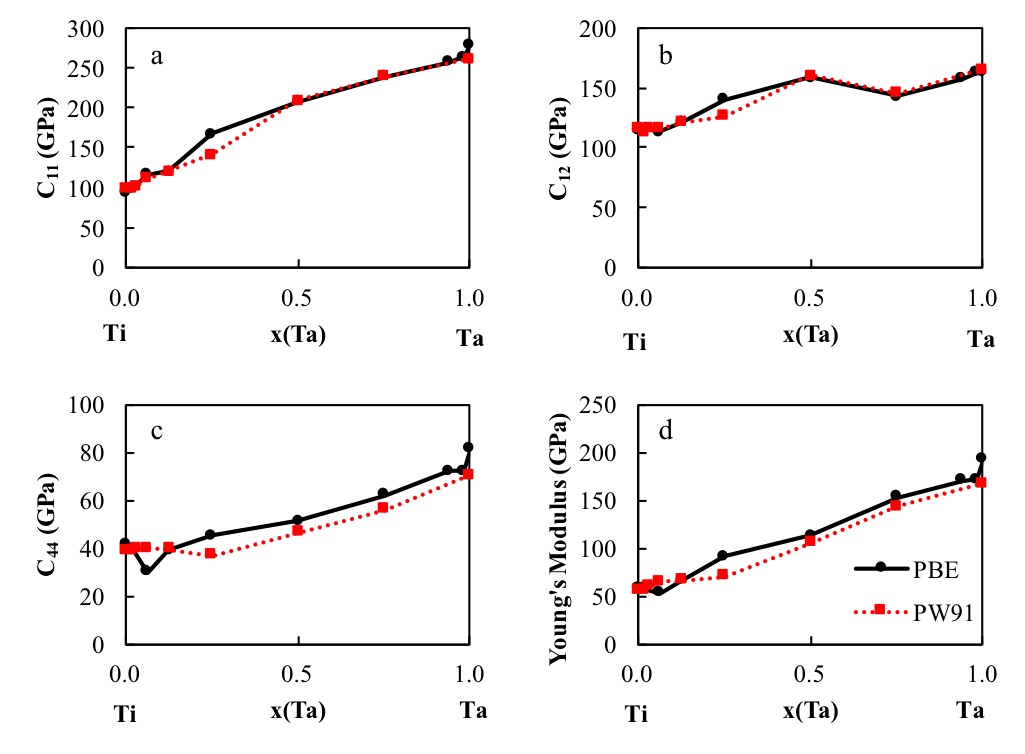
\includegraphics[width=\textwidth]{Chapter-2/Figures/PBEvsPW91.png}
	\caption{Elastic stiffness constants of the bcc Ti-Ta binary system calculated with the GGA and PBE exchange correction functions, respectively.}
	\label{Ch2-figure:PBEvsPW91}
\end{figure}
